\documentclass[12pt, a4paper]{article}

% Pakiety językowe i kodowanie
\usepackage[utf8]{inputenc}
\usepackage[T1]{fontenc}
\usepackage[polish]{babel}

% Pakiety matematyczne i graficzne
\usepackage{amsmath}
\usepackage{amsfonts}
\usepackage{graphicx}
\usepackage{float}
\usepackage{geometry}
\usepackage{hyperref}

% Ustawienia marginesów
\geometry{margin=2.5cm}

% Ustawienia linków
\hypersetup{
    colorlinks=true,
    linkcolor=blue,
    filecolor=magenta,      
    urlcolor=cyan,
    citecolor=green,
    pdftitle={Sprawozdanie - Metody Sztucznej Inteligencji},
}

\title{\textbf{Inteligencja obliczeniowa i jej zastosowania - sprawozdanie}}
\author{Jakub Jaśków, Justyna Ziemichód}
\date{\today}

\begin{document}

\maketitle
\tableofcontents
\newpage

\section{Wstęp}
Niniejsze sprawozdanie prezentuje przekrojową realizację pięciu zadań projektowych z zakresu uczenia maszynowego oraz metod probabilistycznych. W ramach projektu zaimplementowano i poddano analizie następujące problemy:
\begin{enumerate}
    \item \textbf{Grupowanie:} podział wielowymiarowego zbioru \textit{Wine} metodami $k$-means i $k$-medoids (zad. 1.a).
    \item \textbf{Metoda Monte Carlo:} estymacja stałej matematycznej $\pi$ (zad. 2.a) oraz obliczanie całek oznaczonych na przykładzie funkcji sinus (zad. 2.b).
    \item \textbf{Naiwny Klasyfikator Bayesa:} klasyfikacja ciągłych danych biologicznych na zbiorze \textit{Iris} (zad. 3.a) oraz kategoryzacja tekstu na korpusie wiadomości SMS Spam (zad. 3.b).
\end{enumerate}

\section{Środowisko i narzędzia}
Wszystkie algorytmy i analizy zrealizowano w języku \textbf{Python (wersja 3.13)} w izolowanym środowisku wirtualnym (\textit{venv}). Wykorzystano następujące pakiety biblioteczne \cite{scikit-learn}:
\begin{itemize}
    \item \textbf{NumPy \& Pandas:} do operacji wektorowych, optymalizacji obliczeń oraz strukturyzacji zestawów danych.
    \item \textbf{Scikit-Learn:} do implementacji algorytmów uczenia maszynowego (K-means, Naive Bayes), wektoryzacji tekstu (CountVectorizer) i metryk ewaluacyjnych.
    \item \textbf{Matplotlib \& Seaborn:} do realizacji zjawiskowej Eksploracyjnej Analizy Danych (EDA) oraz generowania wykresów naukowych.
\end{itemize}

% ==========================================
% ZADANIE 1
% ==========================================
\section{Zadanie 1: Grupowanie danych}

\subsection{Zadanie 1.a: Algorytmy $k$-means oraz $k$-medoids}
Grupowanie (klasteryzacja) to technika uczenia nienadzorowanego, której celem jest podział obiektów na homogeniczne grupy. Eksperyment przeprowadzono na klasycznym zbiorze \textit{Wine} \cite{uci-wine}, pochodzącym z repozytorium UCI Machine Learning. Zbiór ten zawiera \textbf{178 próbek} reprezentujących trzy różne odmiany winorośli, z których każdą opisuje \textbf{13 cech fizykochemicznych} (m.in. zawartość alkoholu, kwasowość, magnez).

Aby optymalnie dobrać liczbę klastrów ($k$), przed uruchomieniem algorytmów wykonano analizę dwiema metodami numerycznymi: metodą łokcia oraz wskaźnikiem Silhouette.

\begin{figure}[H]
    \centering
    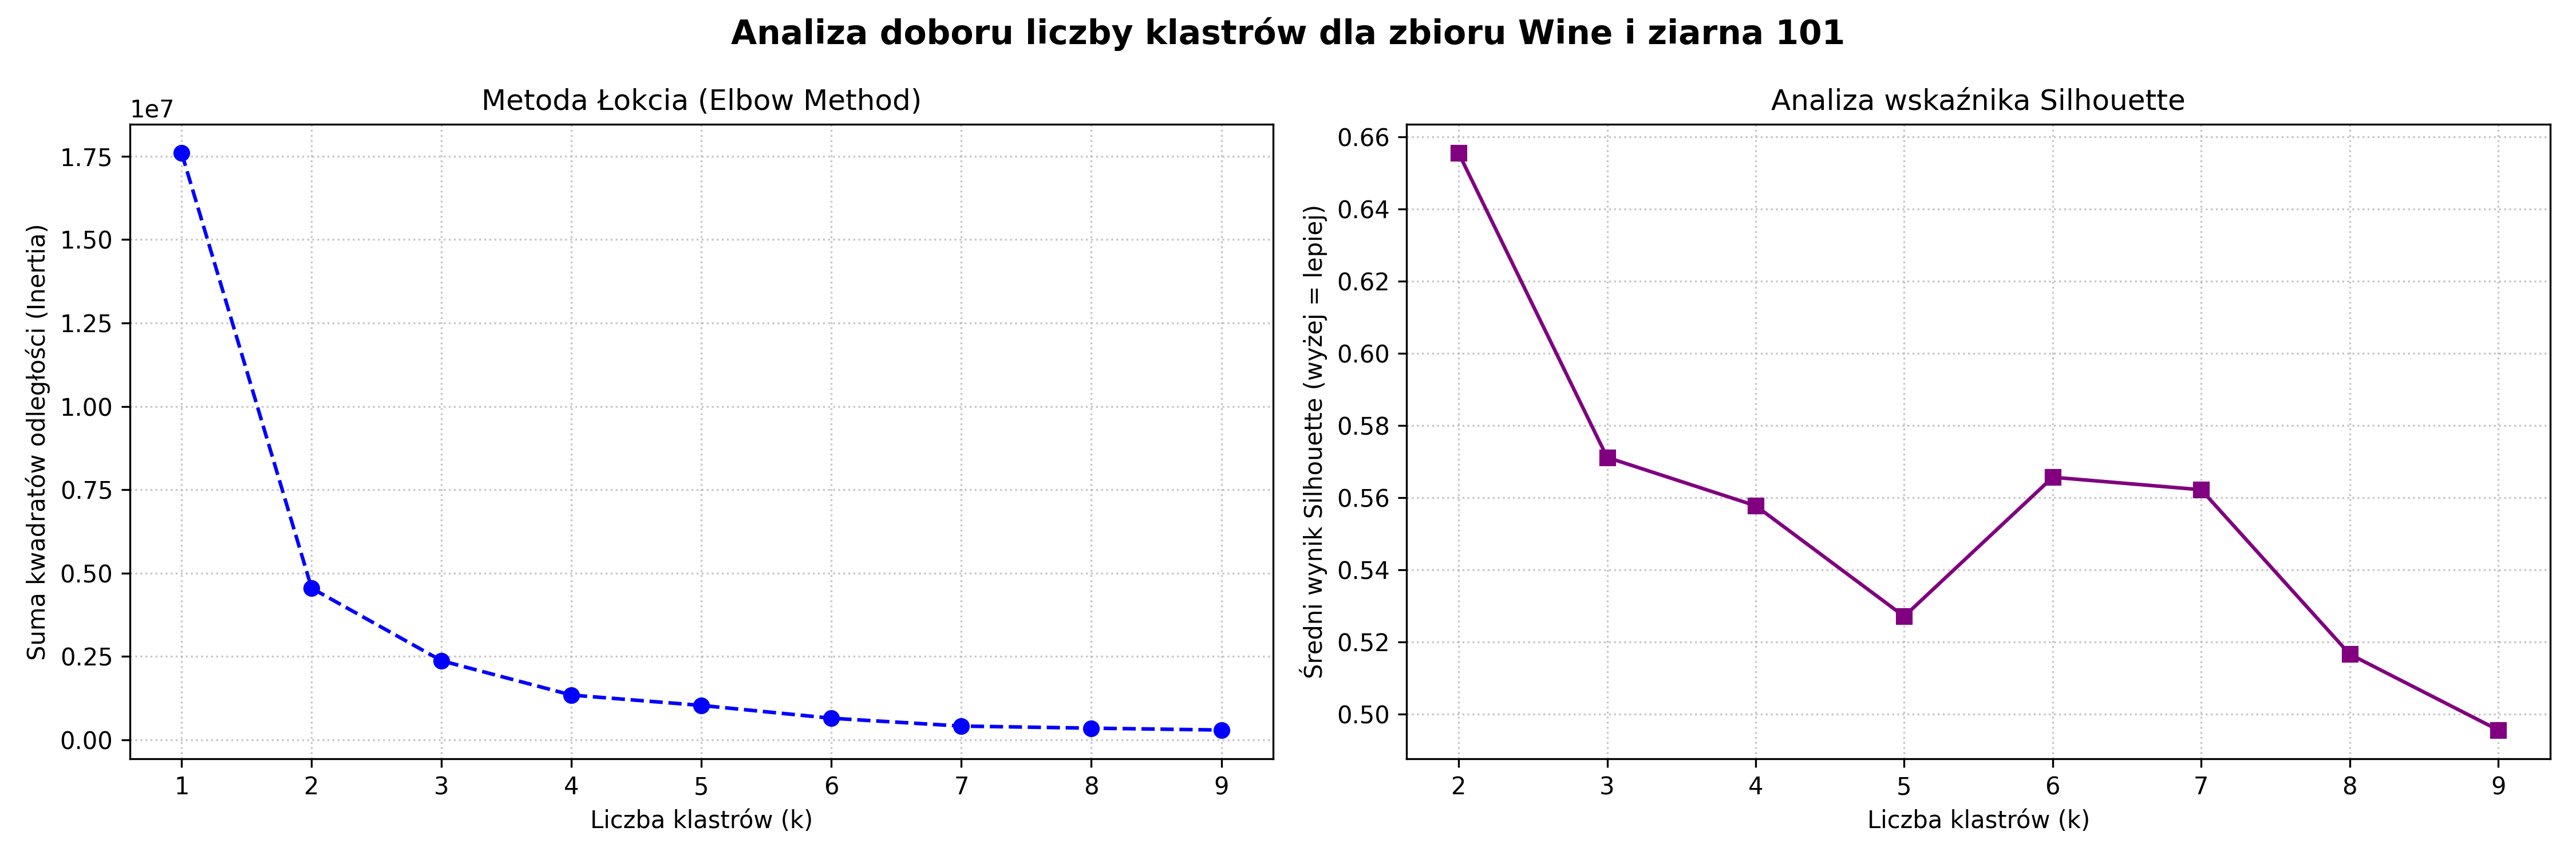
\includegraphics[width=\textwidth]{img/clustering_analysis_seed_101.png}
    \label{fig:analysis}
\end{figure}

Na Rysunku \ref{fig:analysis} przedstawiono wyniki doboru optymalnej liczby klastrów. Wykres po lewej stronie (metoda łokcia) wykazuje wyraźny punkt przegięcia dla $k=3$, co znajduje odzwierciedlenie w analizie wskaźnika Silhouette po prawej stronie, gdzie dla tej samej liczby klastrów odnotowano wysoki wynik spójności. Przyjęto zatem ostateczny podział na 3 klastry, co idealnie pokrywa się z faktyczną liczbą klas w badanym zbiorze danych.

\begin{figure}[H]
    \centering
    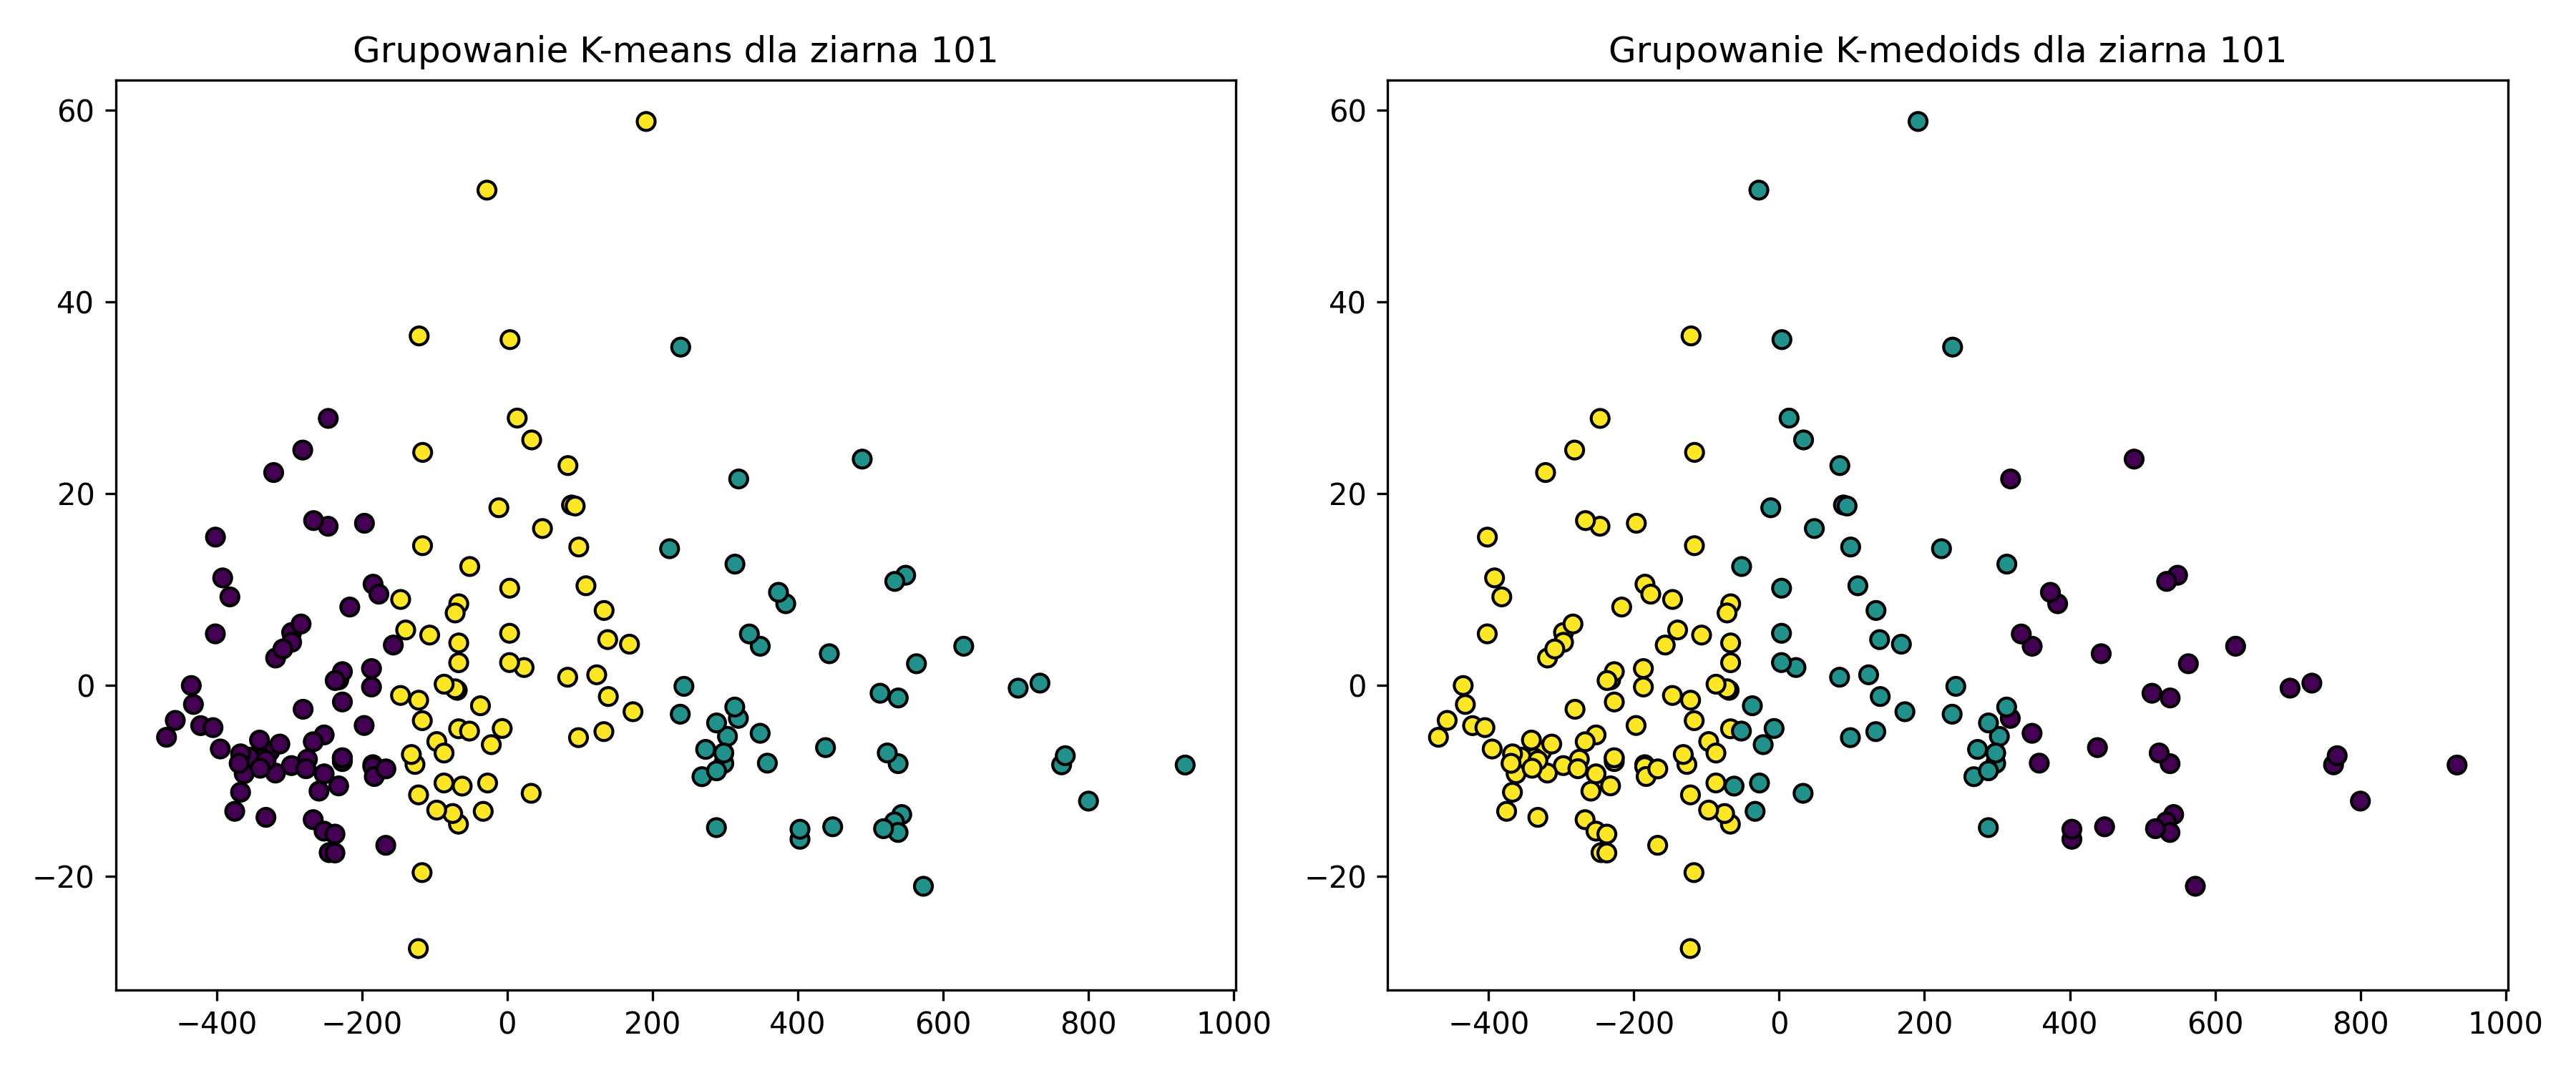
\includegraphics[width=0.9\textwidth]{img/clustering_101.png}
    \caption{Porównanie grupowania: $k$-means vs $k$-medoids.}
    \label{fig:clustering}
\end{figure}

Rysunek \ref{fig:clustering} przedstawia wynik segmentacji w przestrzeni zredukowanej do dwóch wymiarów przy użyciu algorytmu PCA (Principal Component Analysis). Oba algorytmy wydzieliły trzy podobne obszary decyzyjne. Algorytm $k$-medoids \cite{kmedoids}, z uwagi na konieczność wyboru rzeczywistego punktu danych jako centrum medoidy, utworzył nieznacznie inne granice w obszarach nakładania się klastrów w porównaniu do $k$-means, który operuje na abstrakcyjnych środkach ciężkości (centroidach).

% ==========================================
% ZADANIE 2
% ==========================================
\section{Zadanie 2: Metody Monte Carlo}

\subsection{Zadanie 2.a: Obliczanie stałej $\pi$}
Metody Monte Carlo \cite{montecarlo} wykorzystują generowanie liczb pseudolosowych do rozwiązywania problemów numerycznych i fizycznych. W estymacji stałej $\pi$ posłużono się eksperymentem geometrycznym polegającym na wpisaniu pełnego koła o promieniu $r=1$ w kwadrat o boku $a=2$. Stosunek pola koła do pola kwadratu wynosi $\frac{\pi}{4}$.

\begin{figure}[H]
    \centering
    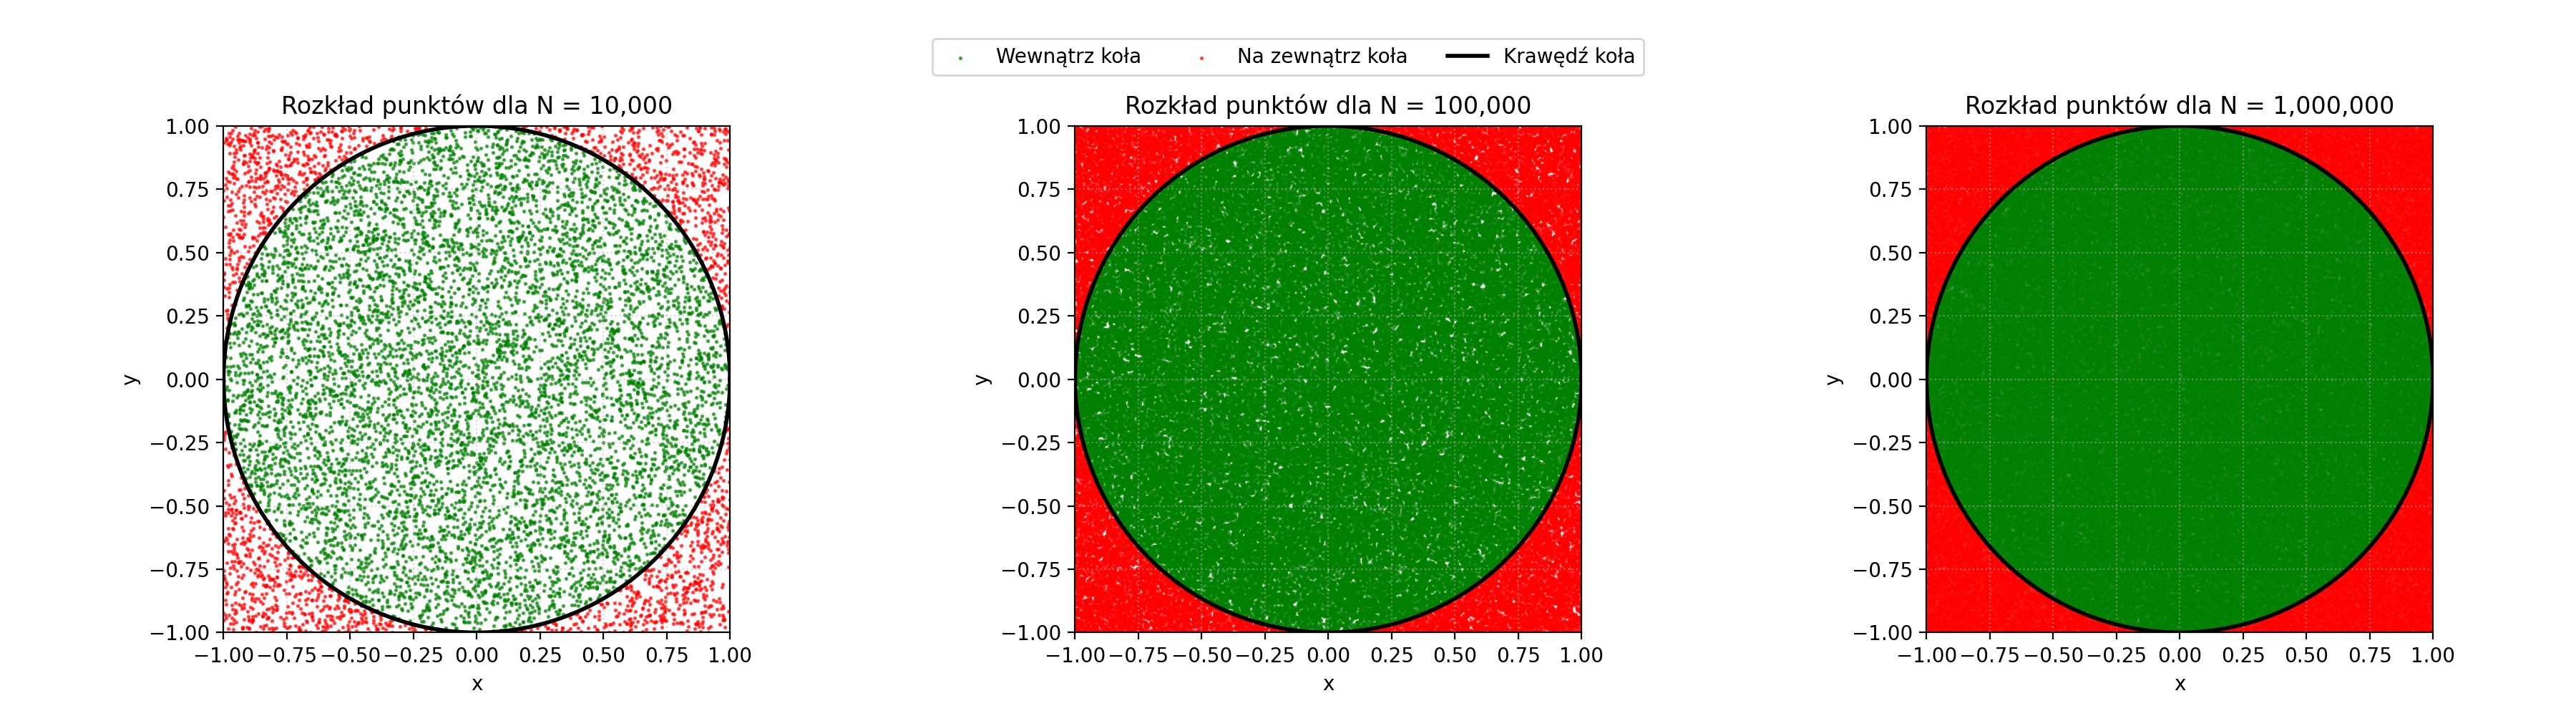
\includegraphics[width=\textwidth]{img/pi_monte_carlo_combined.png}
    \caption{Rozkład punktów wewnątrz i na zewnątrz koła dla trzech różnych rzędów wielkości próby ($N$).}
    \label{fig:pi_scatter}
\end{figure}

Losując współrzędne wzdłuż rozkładu jednostajnego na przedziale $[-1, 1]$, sprawdzano warunek przynależności do figury ($x^2 + y^2 \le 1$). Symulację przeprowadzono w trzech scenariuszach zagęszczenia punktów: dla $N = 10^4, 10^5$ oraz $10^6$ (Rys. \ref{fig:pi_scatter}). Zgodnie z prawem wielkich liczb, stosunek punktów trafionych wewnątrz okręgu do wszystkich wylosowanych punktów przemnożony przez 4 przybliżał wartość stałej Archimedesa.

\begin{figure}
    \centering
    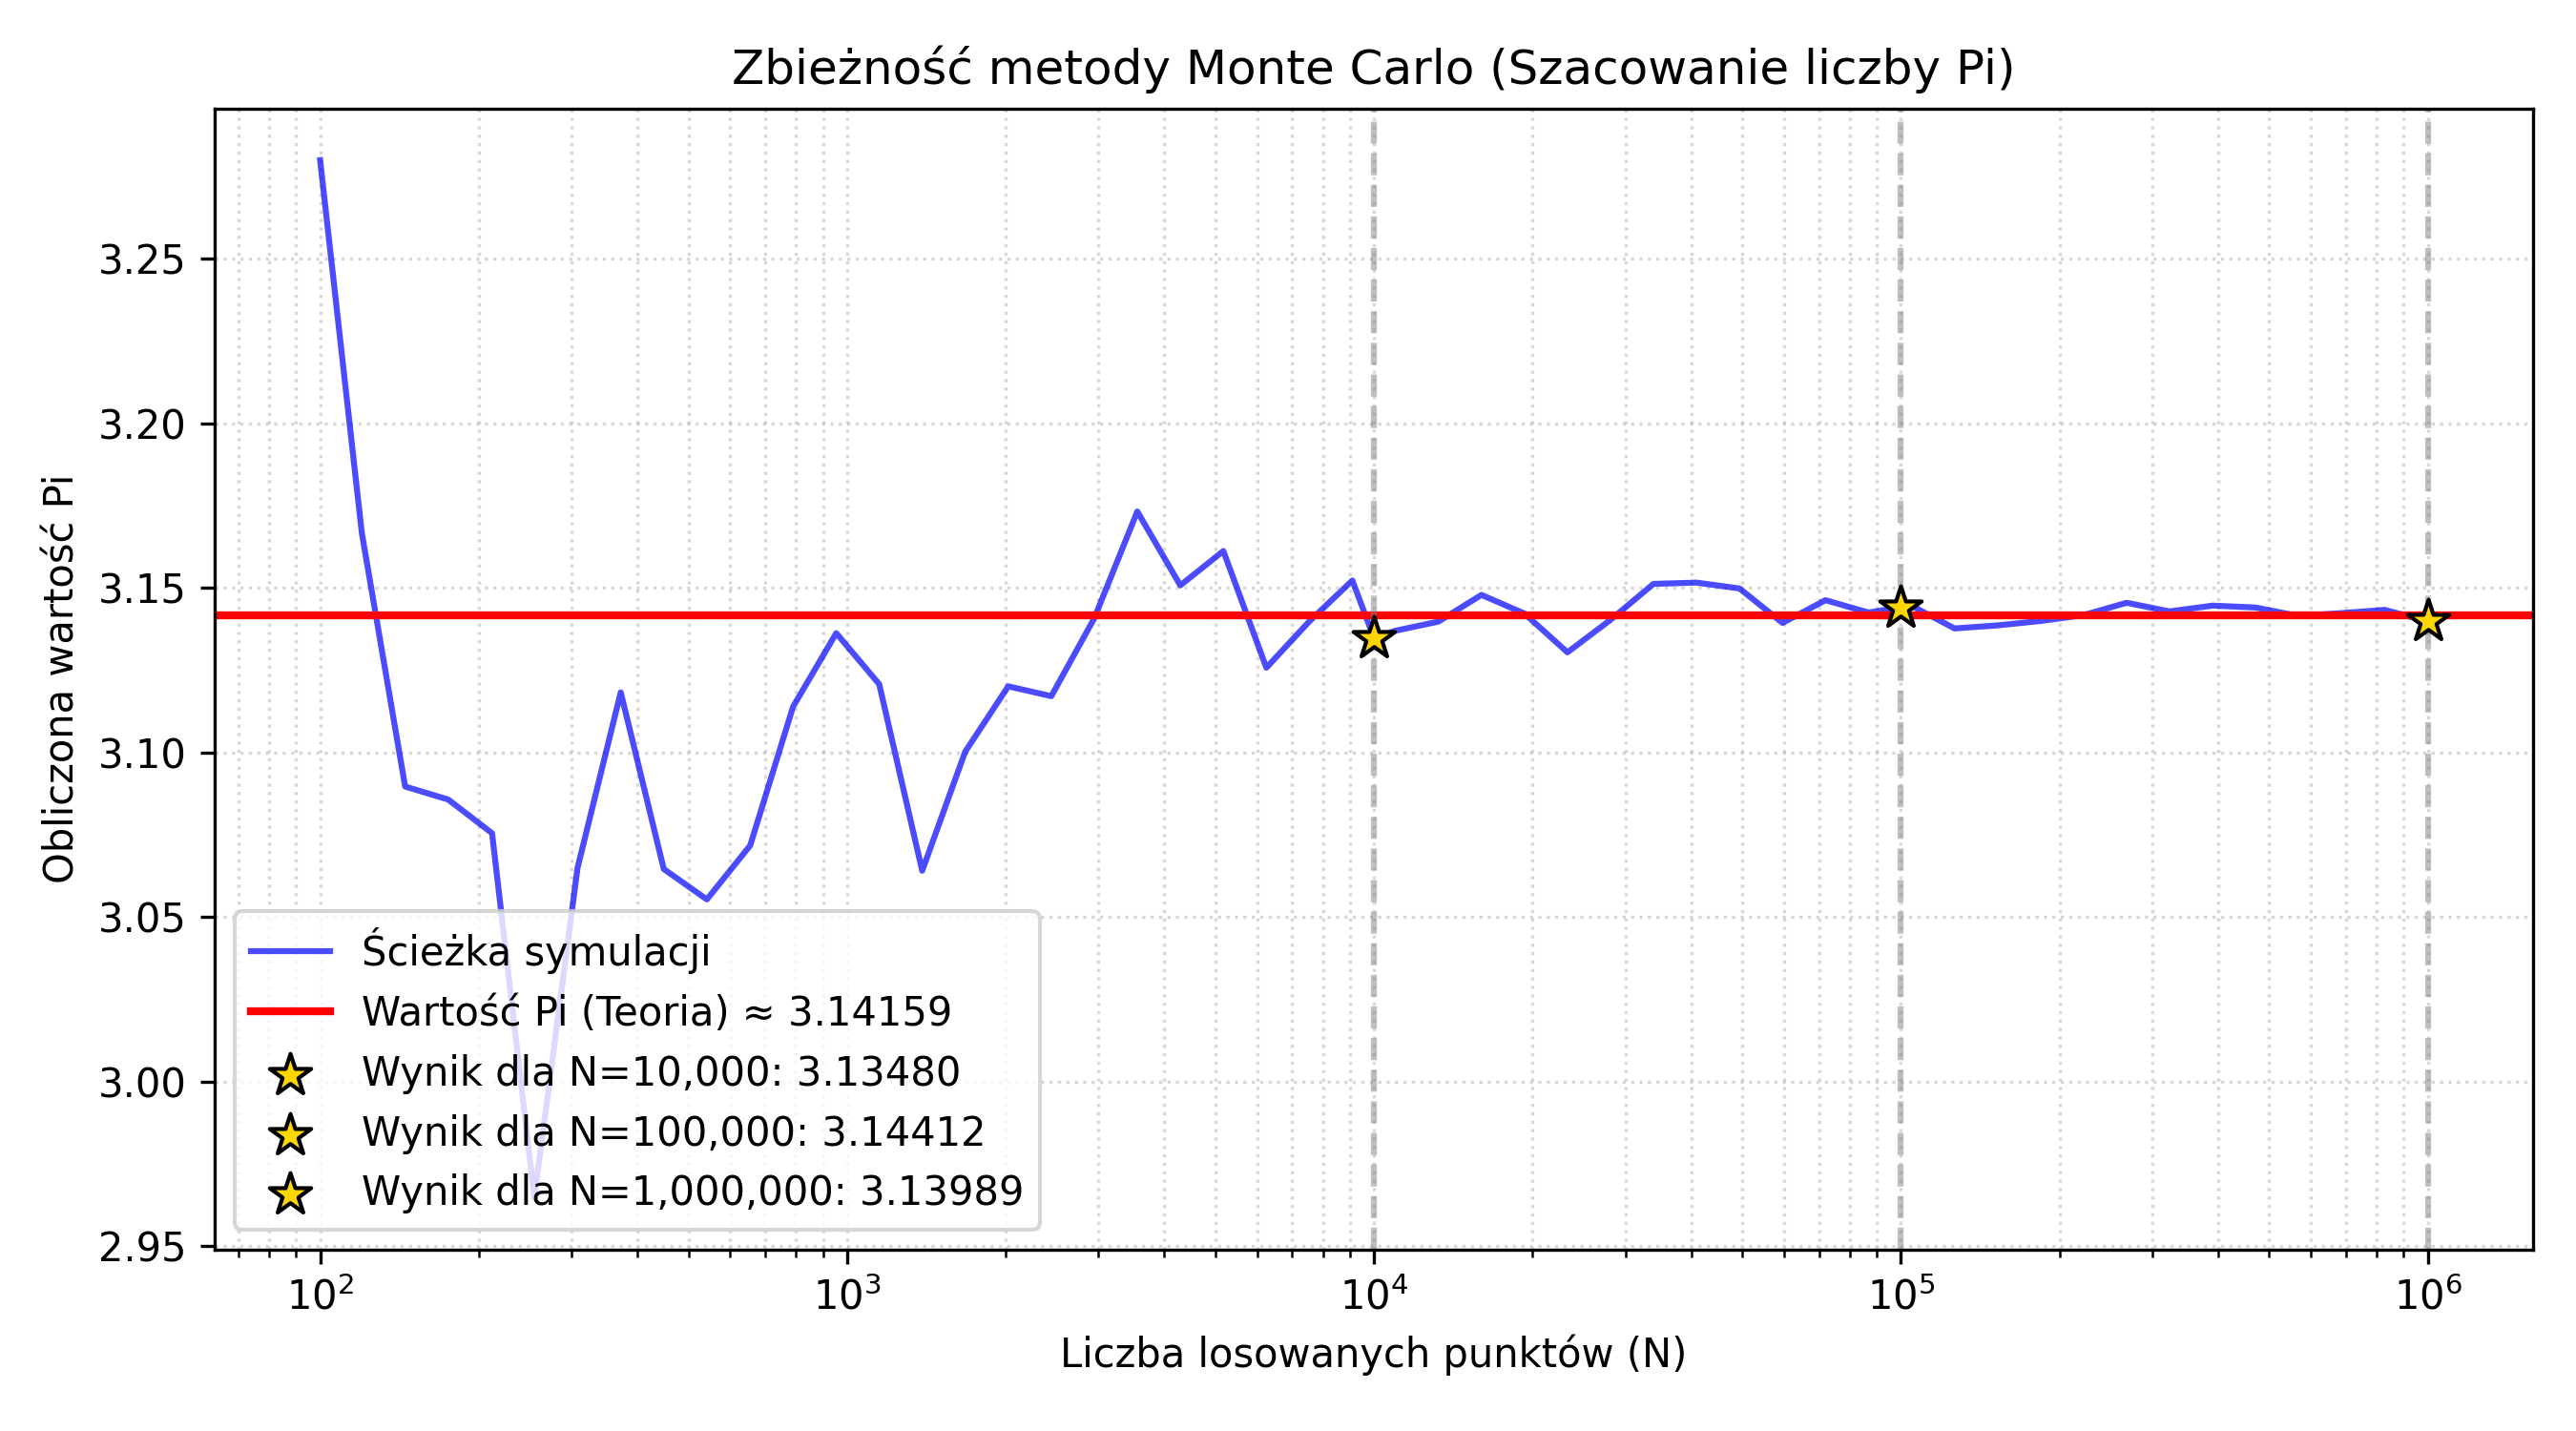
\includegraphics[width=0.9\textwidth]{img/pi_mc_convergence.png}
    \caption{Zbieżność estymatora $\pi$ (skala logarytmiczna).}
    \label{fig:pi_conv}
\end{figure}


\begin{figure}
    \centering
    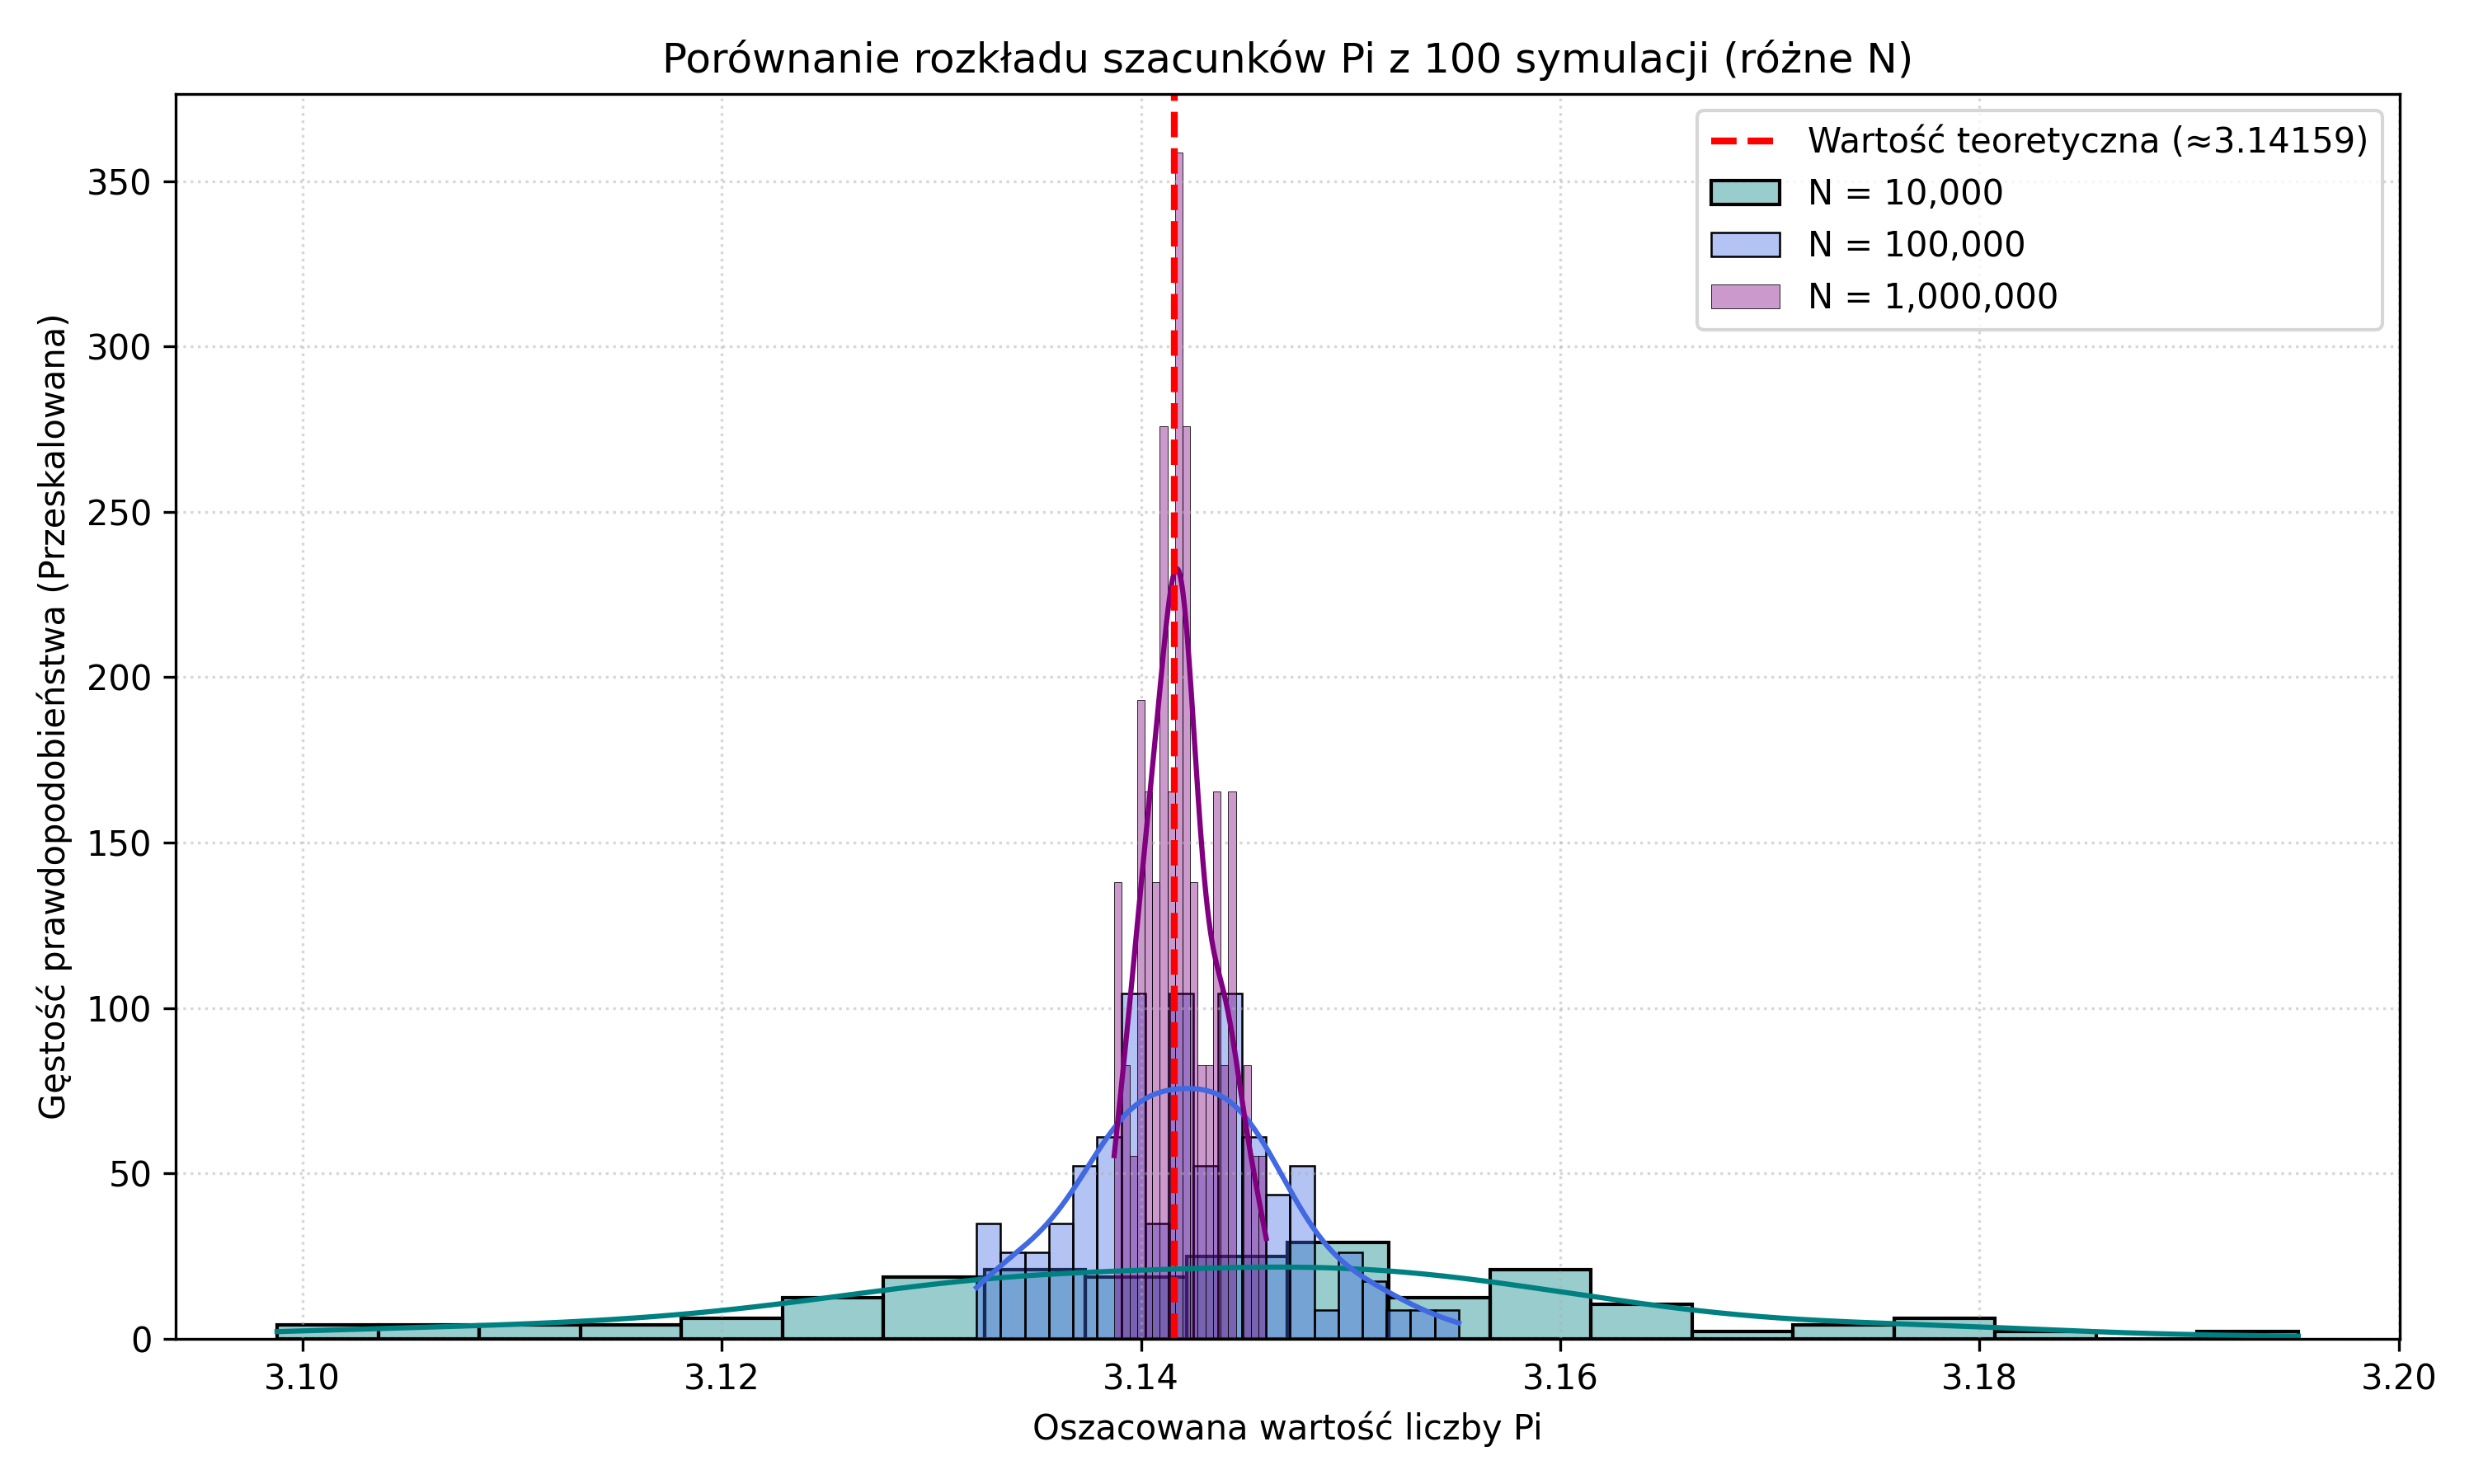
\includegraphics[width=0.9\textwidth]{img/pi_mc_histogram.png}
    \caption{Zagęszczenie rozkładu wyników (100 symulacji dla każdego $N$).}
    \label{fig:pi_hist}
\end{figure}

Wykres \ref{fig:pi_conv} udowadnia, że wraz ze wzrostem liczby prób ($N$), estymator stabilizuje się i asymptotycznie dąży do wartości teoretycznej $\pi \approx 3.14159$. Dodatkowo, analiza stochastyczna (Rys. \ref{fig:pi_hist}) ukazuje proces zwężania się wariancji. Wielokrotne powtórzenie eksperymentu potwierdza, że zwiększenie rzędu wielkości próby prowadzi do silniejszego skupienia wyników wokół wartości oczekiwanej, redukując błąd estymacji na mocy Centralnego Twierdzenia Granicznego.

\subsection{Zadanie 2.b: Obliczanie całek oznaczonych}
Algorytm stochastyczny zastosowano również do obliczenia całki z funkcji $f(x) = \sin(x)$ na przedziale $[0, \pi]$. Analityczna wartość docelowa to dokładnie 2.

\begin{figure}[H]
    \centering
    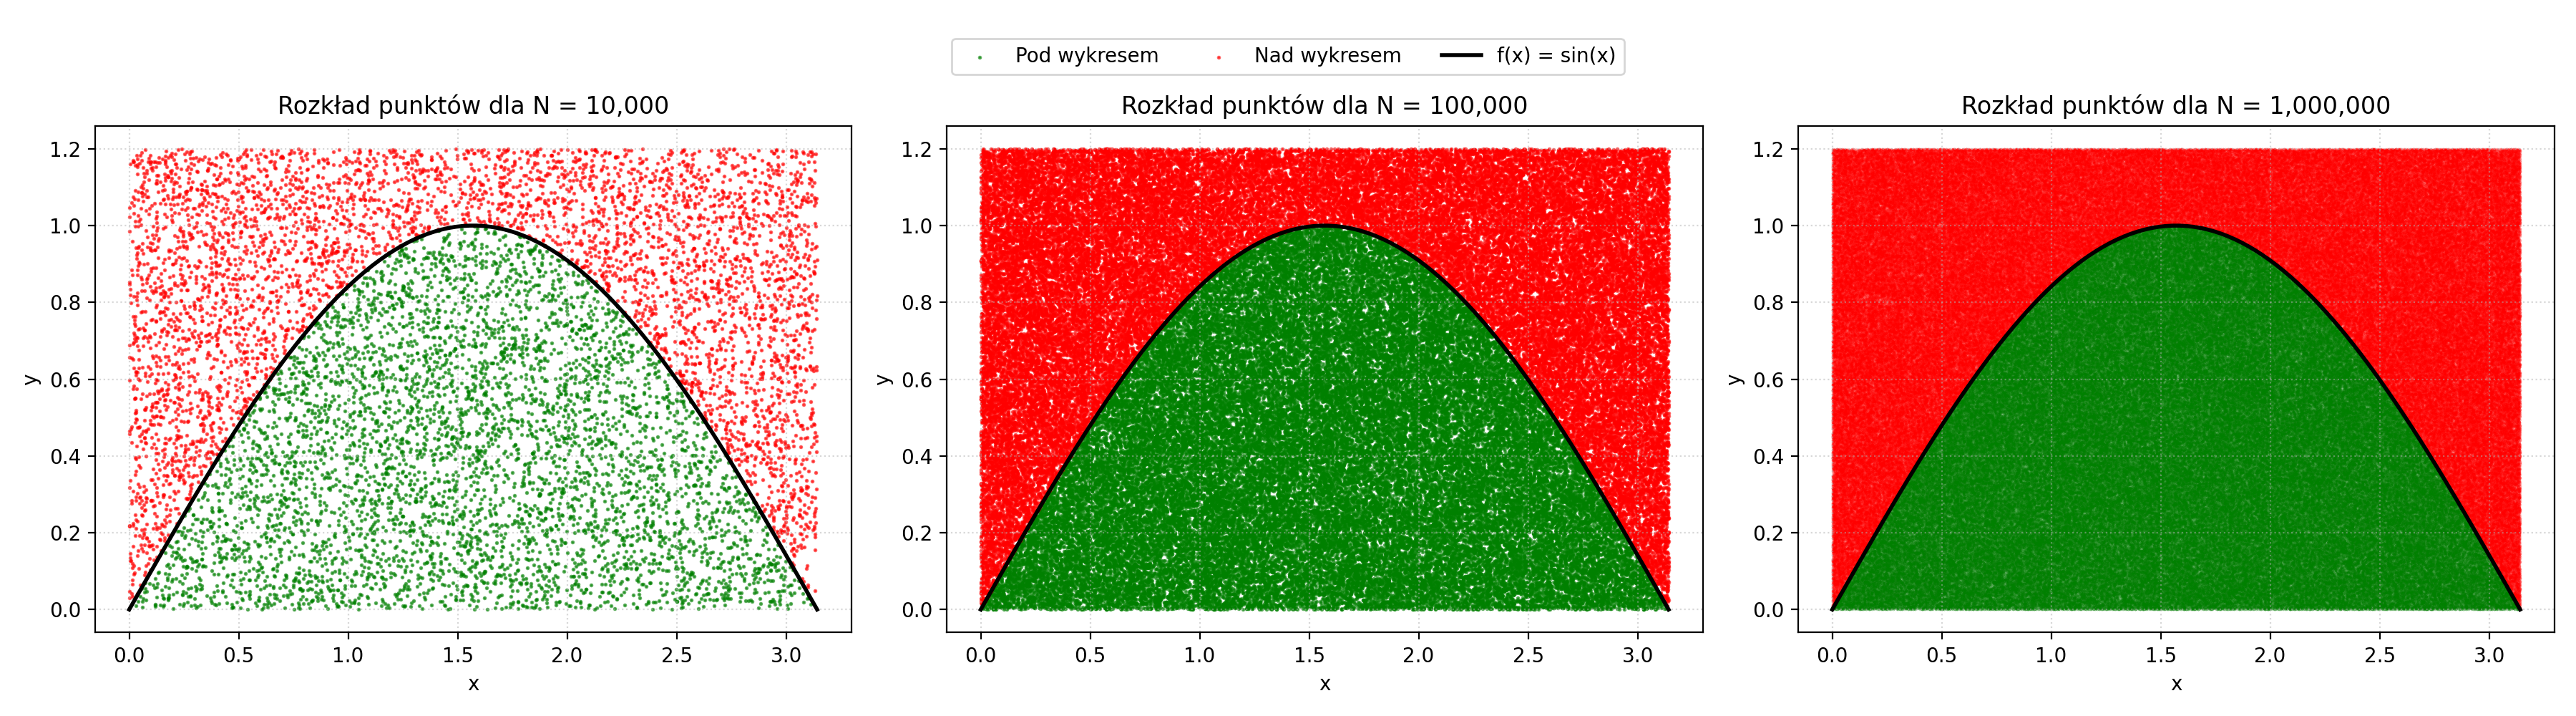
\includegraphics[width=\textwidth]{img/monte_carlo_combined.png}
    \caption{Rozkład punktów pod i nad wykresem funkcji $\sin(x)$ dla trzech różnych rzędów wielkości próby ($N$).}
    \label{fig:mc_integral}
\end{figure}

W obszarze otaczającym funkcję wygenerowano losowe punkty, poddając analizie trzy scenariusze: dla $N = 10^4, 10^5$ oraz $10^6$ (Rys. \ref{fig:mc_integral}). Zgodnie z założeniami metody, obliczona na ich podstawie zintegrowana wartość całki przybliżała się do wartości 2.0, stając się tym precyzyjniejsza, im więcej punktów brało udział w losowaniu.

\begin{figure}
    \centering
    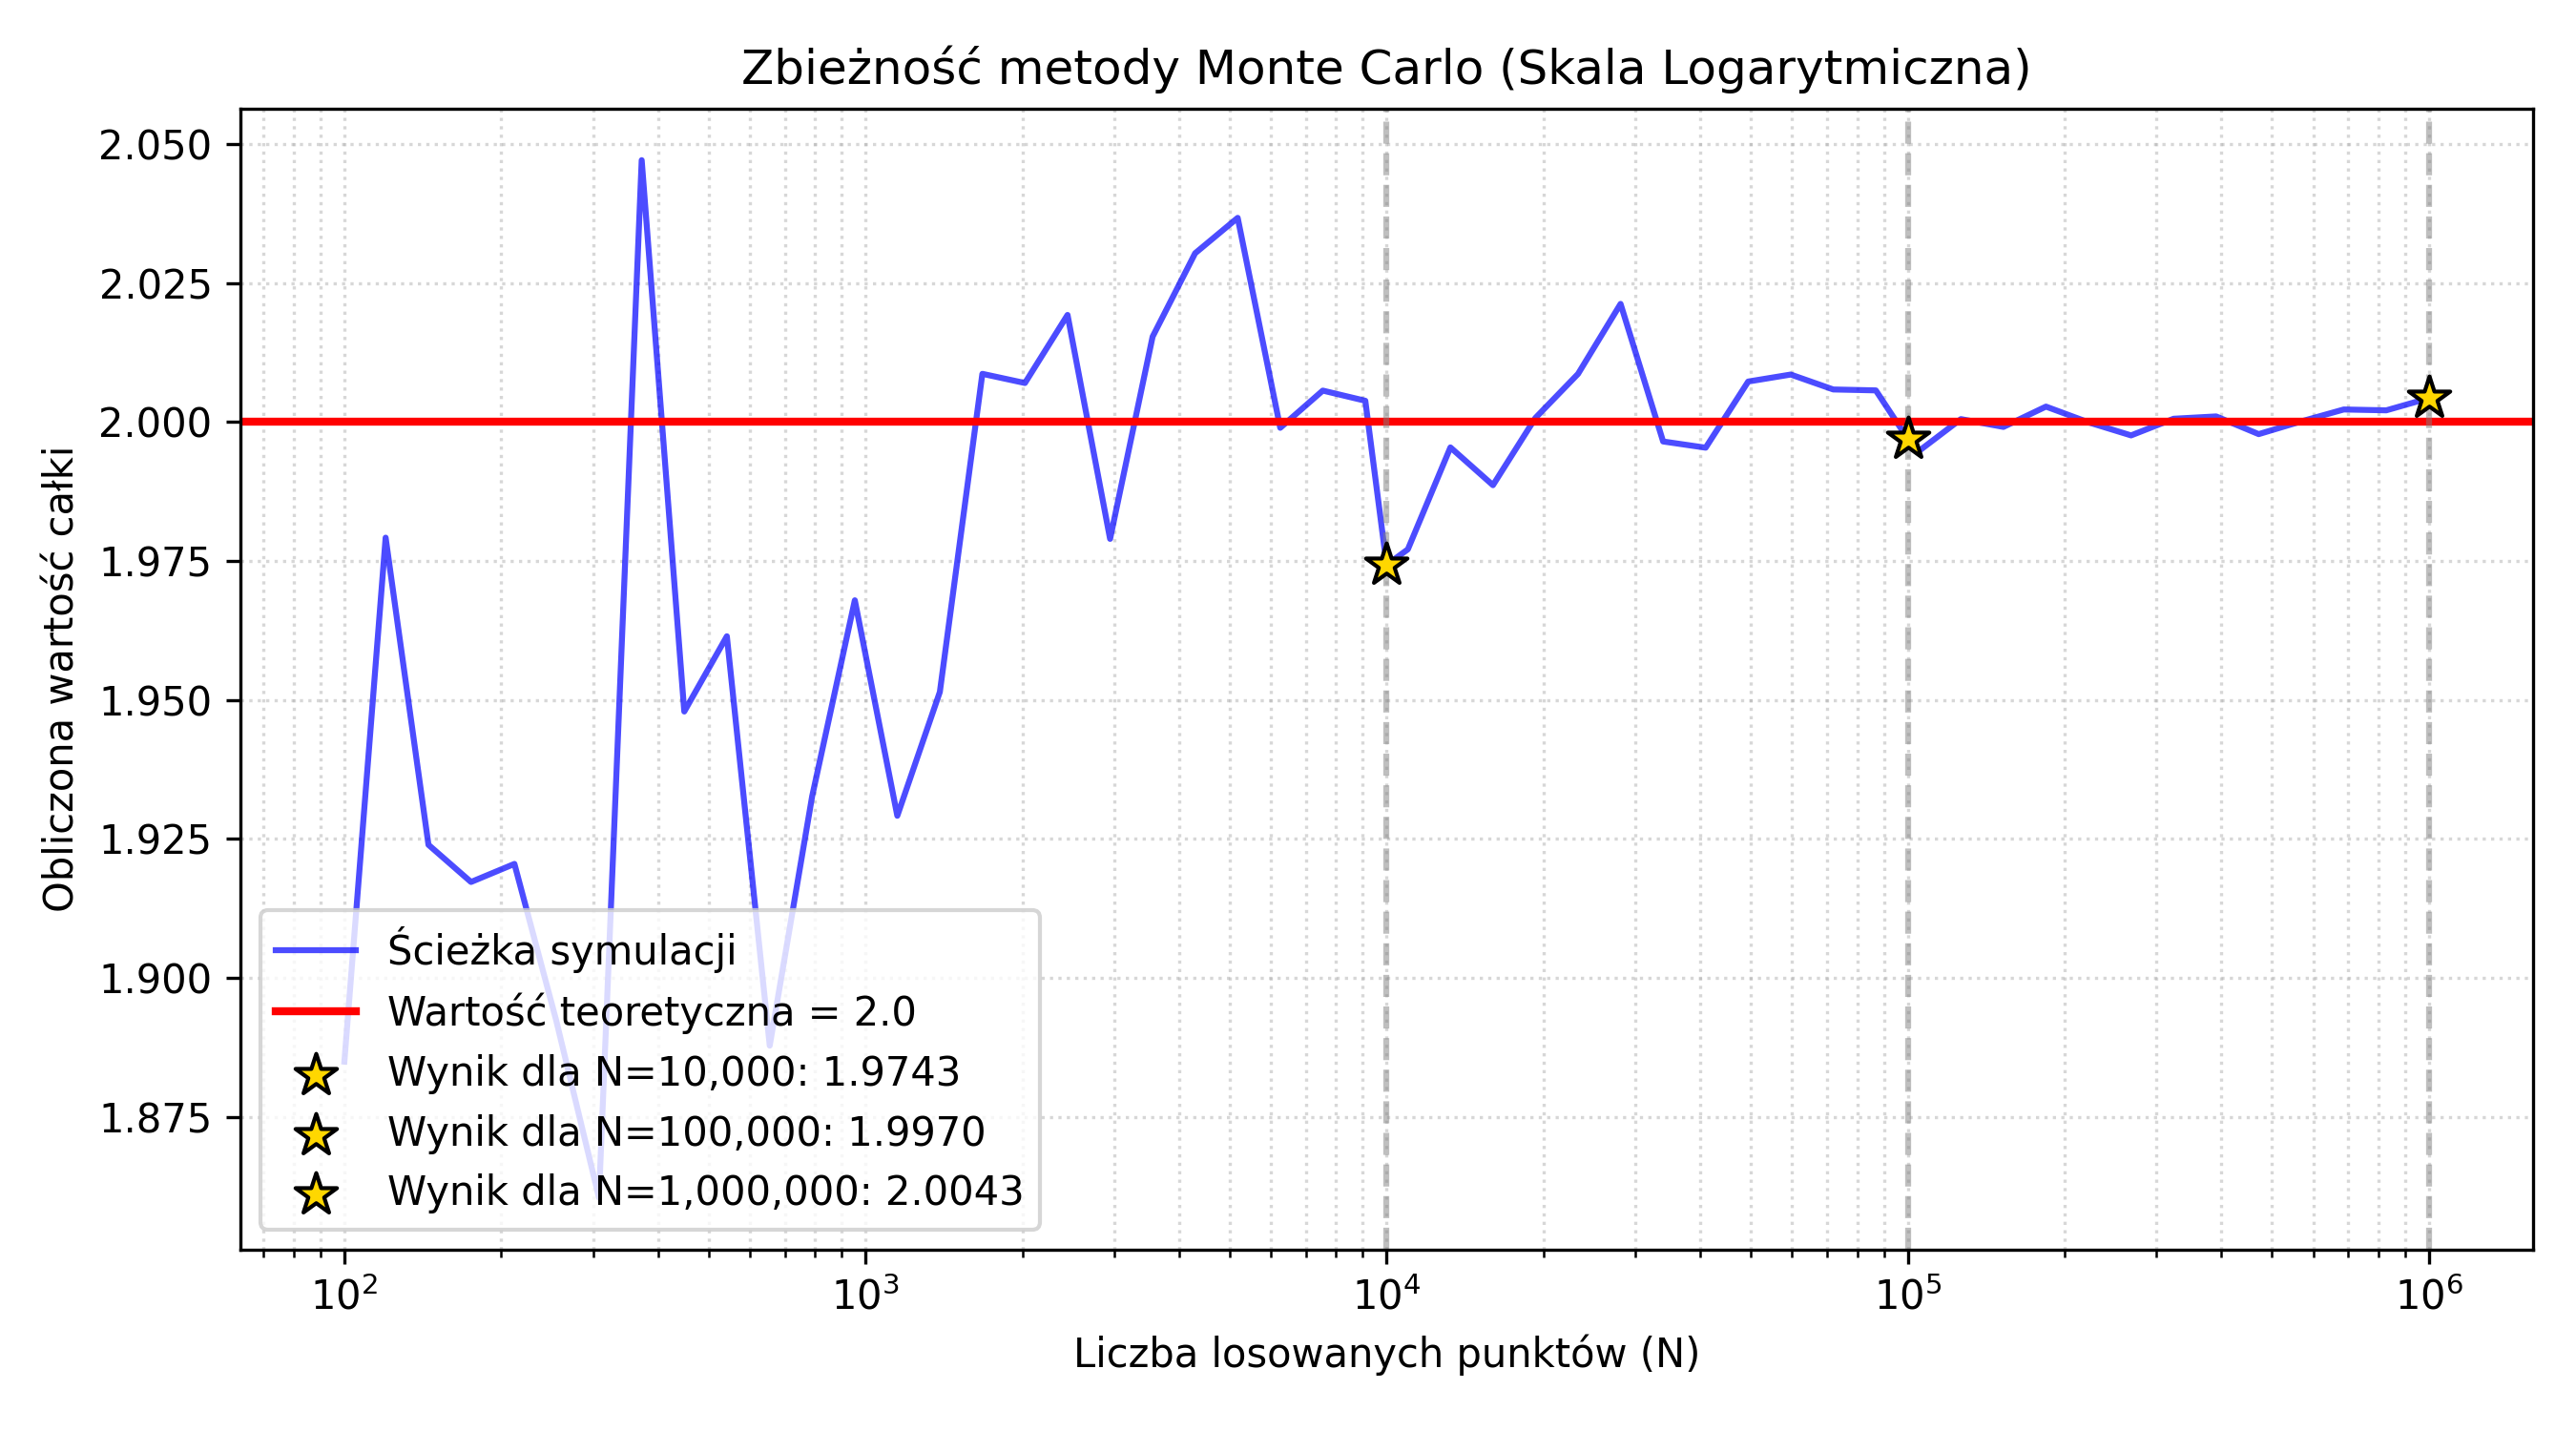
\includegraphics[width=\textwidth]{img/mc_convergence.png}
    \caption{Zbieżność metody Monte Carlo (skala logarytmiczna dla osi N).}
    \label{fig:mc_conv}
\end{figure}

\begin{figure}
        \centering
        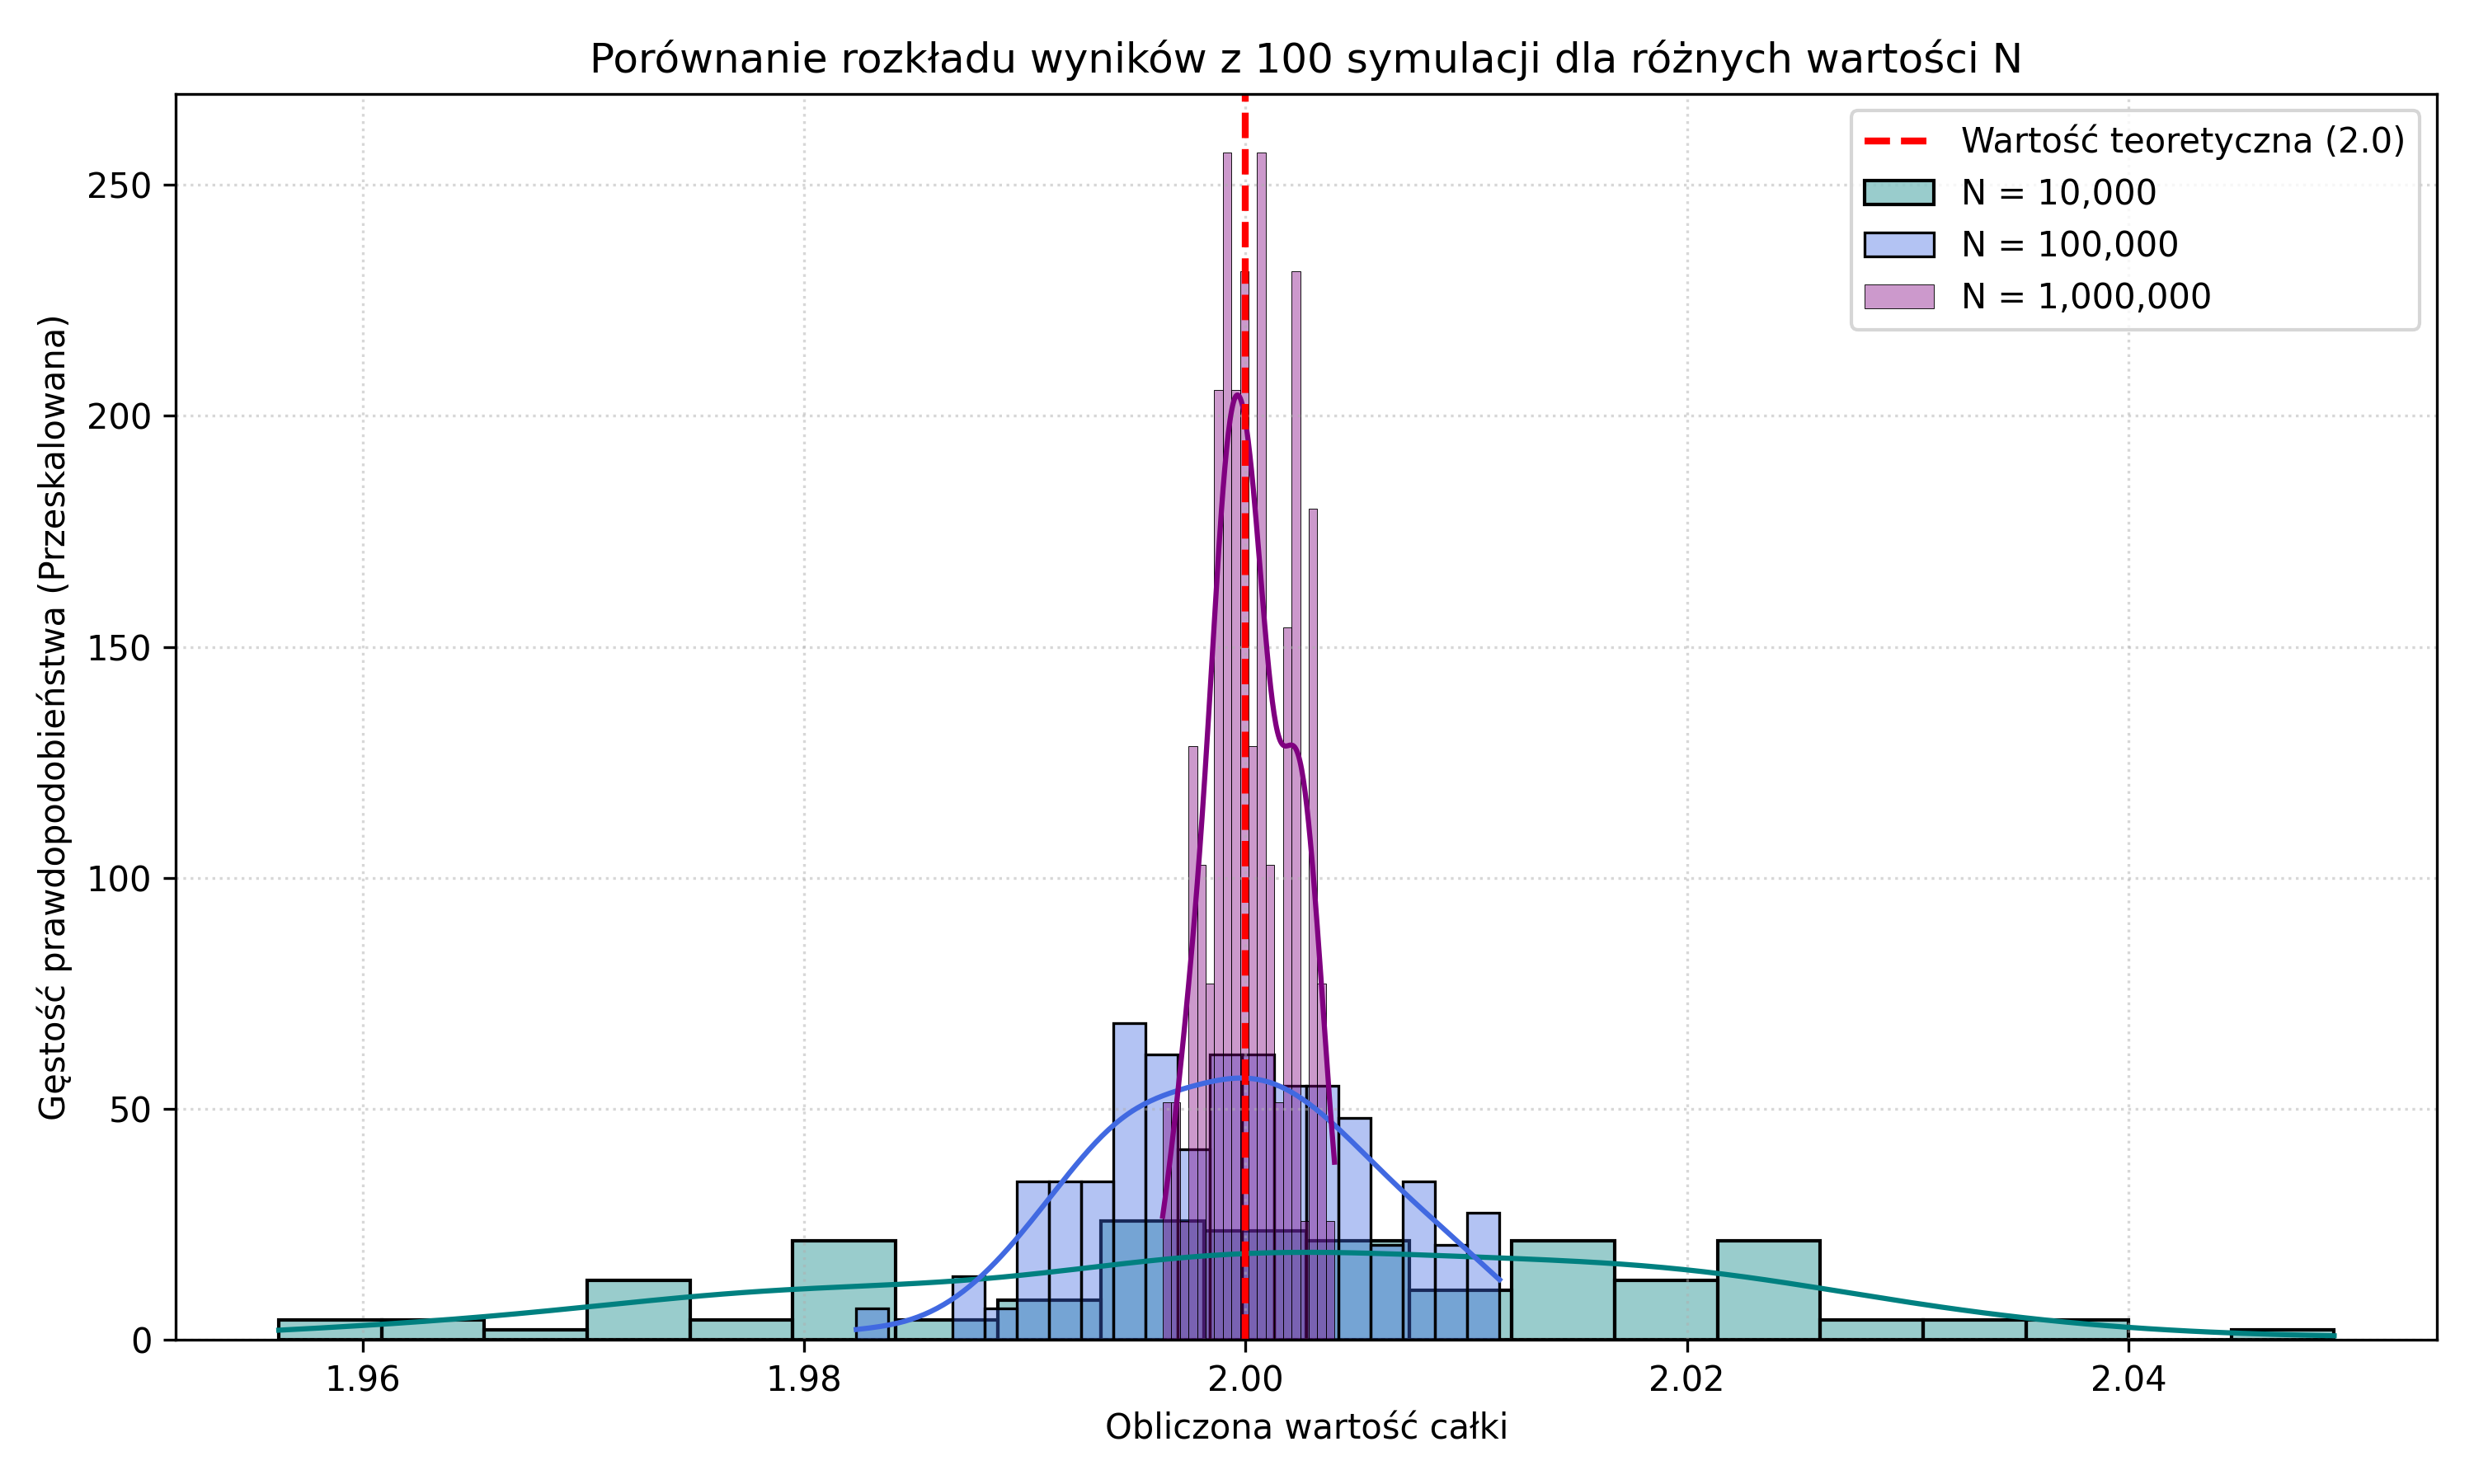
\includegraphics[width=\textwidth]{img/mc_histogram.png}
        \caption{Zagęszczenie rozkładu wyników (100 symulacji dla każdego $N$).}
        \label{fig:mc_hist}
\end{figure}

Zbieżność metody została szerzej zobrazowana na Rysunku \ref{fig:mc_conv}, gdzie za pomocą skali logarytmicznej przedstawiono ewolucję błędu szacowania. Dodatkowa analiza stochastyczna (Rys. \ref{fig:mc_hist}), oparta na 100-krotnym powtórzeniu eksperymentu dla każdej głównej wartości $N$, pokazuje, że empiryczne wyniki układają się w rozkład bliski normalnemu ze średnią równą teoretycznej wartości 2.0. Widoczne zawężanie się histogramów wokół wartości oczekiwanej przy rosnącym $N$ wskazuje na drastyczny spadek wariancji i błędu estymacji. Zjawisko to bezpośrednio wynika z Centralnego Twierdzenia Granicznego, będącego fundamentem efektywności metody Monte Carlo.
% ==========================================
% ZADANIE 3
% ==========================================
\section{Zadanie 3: Naiwny Klasyfikator Bayesa}

\subsection{Zadanie 3.a: Problem "Irysy" (Dane ciągłe)}
Do klasyfikacji gatunków użyto klasycznego zbioru \textit{Fisher's Iris dataset} z 1936 roku \cite{fisher-iris}. Zbiór składa się z \textbf{150 próbek} (po 50 dla trzech klas: \textit{Setosa, Versicolor, Virginica}) i \textbf{4 atrybutów ciągłych} opisujących wymiary płatków i działek kielicha. Z uwagi na ciągły charakter zmiennych, zastosowano probabilistyczny wariant \textit{Gaussian Naive Bayes}.

\begin{figure}[H]
    \centering
    \begin{minipage}{0.48\textwidth}
        \centering
        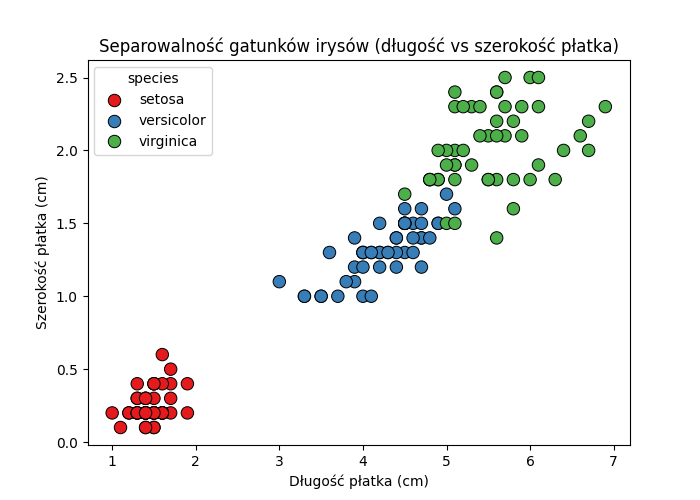
\includegraphics[width=\textwidth]{img/iris_eda.png}
        \caption{Separowalność gatunków irysów.}
        \label{fig:iris_eda}
    \end{minipage}\hfill
    \begin{minipage}{0.48\textwidth}
        \centering
        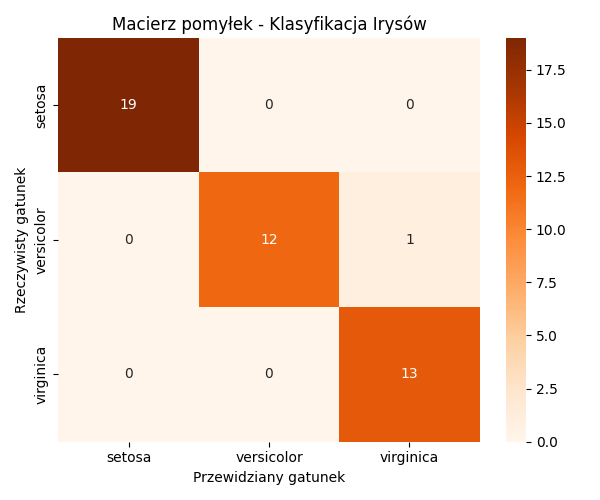
\includegraphics[width=\textwidth]{img/iris_cm.png}
        \caption{Macierz pomyłek modelu.}
        \label{fig:iris_cm}
    \end{minipage}
\end{figure}

Zgodnie z analizą na Rysunku \ref{fig:iris_eda}, klasa \textit{Setosa} jest liniowo odizolowana. Macierz pomyłek (Rysunek \ref{fig:iris_cm}) z ewaluacji zbioru testowego ($30\%$) wykazuje brak błędów modelu na klasie separowalnej oraz pojedyncze przeoczenia na nieliniowej granicy decyzyjnej gatunków \textit{Versicolor} i \textit{Virginica}, co przekłada się na ostateczną dokładność rzędu $97\%$.

\subsection{Zadanie 3.b: Filtrowanie spamu (Klasyfikacja tekstu)}
Weryfikacją modelu dla danych dyskretnych (liczności tokenów) było rozpoznawanie spamu z użyciem korpusu \textit{SMS Spam Collection} \cite{sms-spam}. Zbiór zawiera \textbf{5572 wiadomości tekstowe}, z czego 86.6\% to wiadomości legalne (Ham), a 13.4\% to Spam (jest to zbiór mocno niezbalansowany). Zastosowano metodologię wektoryzacji tekstu \textit{Bag-of-Words} oraz \textit{Multinomial Naive Bayes}.

\begin{figure}[H]
    \centering
    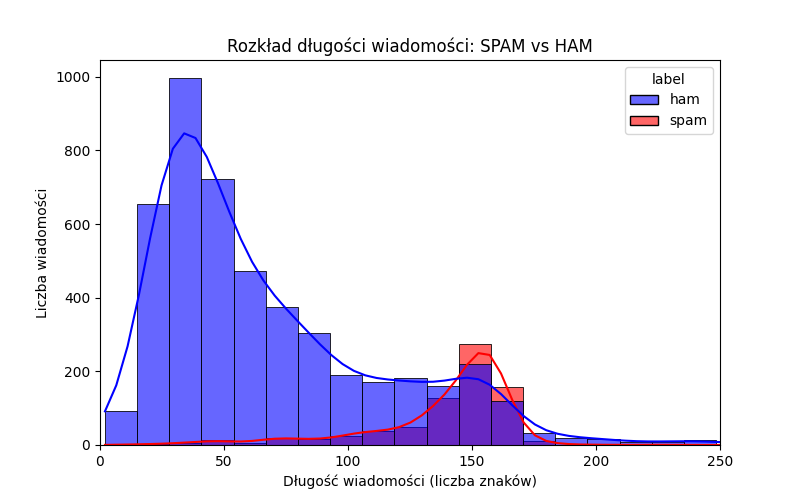
\includegraphics[width=0.65\textwidth]{img/spam_length_dist.png}
    \caption{Rozkład długości wiadomości SMS z podziałem na klasy.}
    \label{fig:spam_len}
\end{figure}

Eksploracja danych (Rysunek \ref{fig:spam_len}) potwierdza, iż wiadomości sklasyfikowane jako spam wykazują wyższą średnią liczbę znaków. 

\begin{figure}[H]
    \centering
    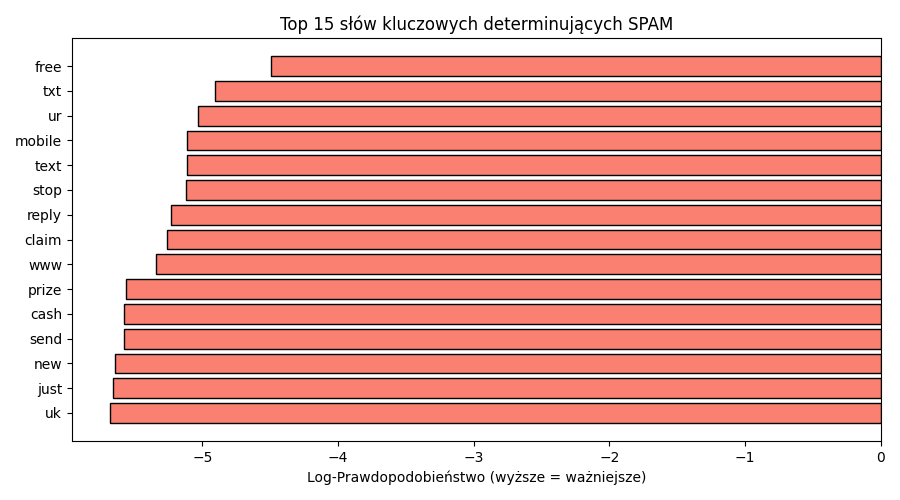
\includegraphics[width=0.6\textwidth]{img/real_spam_features.png}
    \caption{Najważniejsze słowa kluczowe (SPAM).}
    \label{fig:spam_feat}
    
    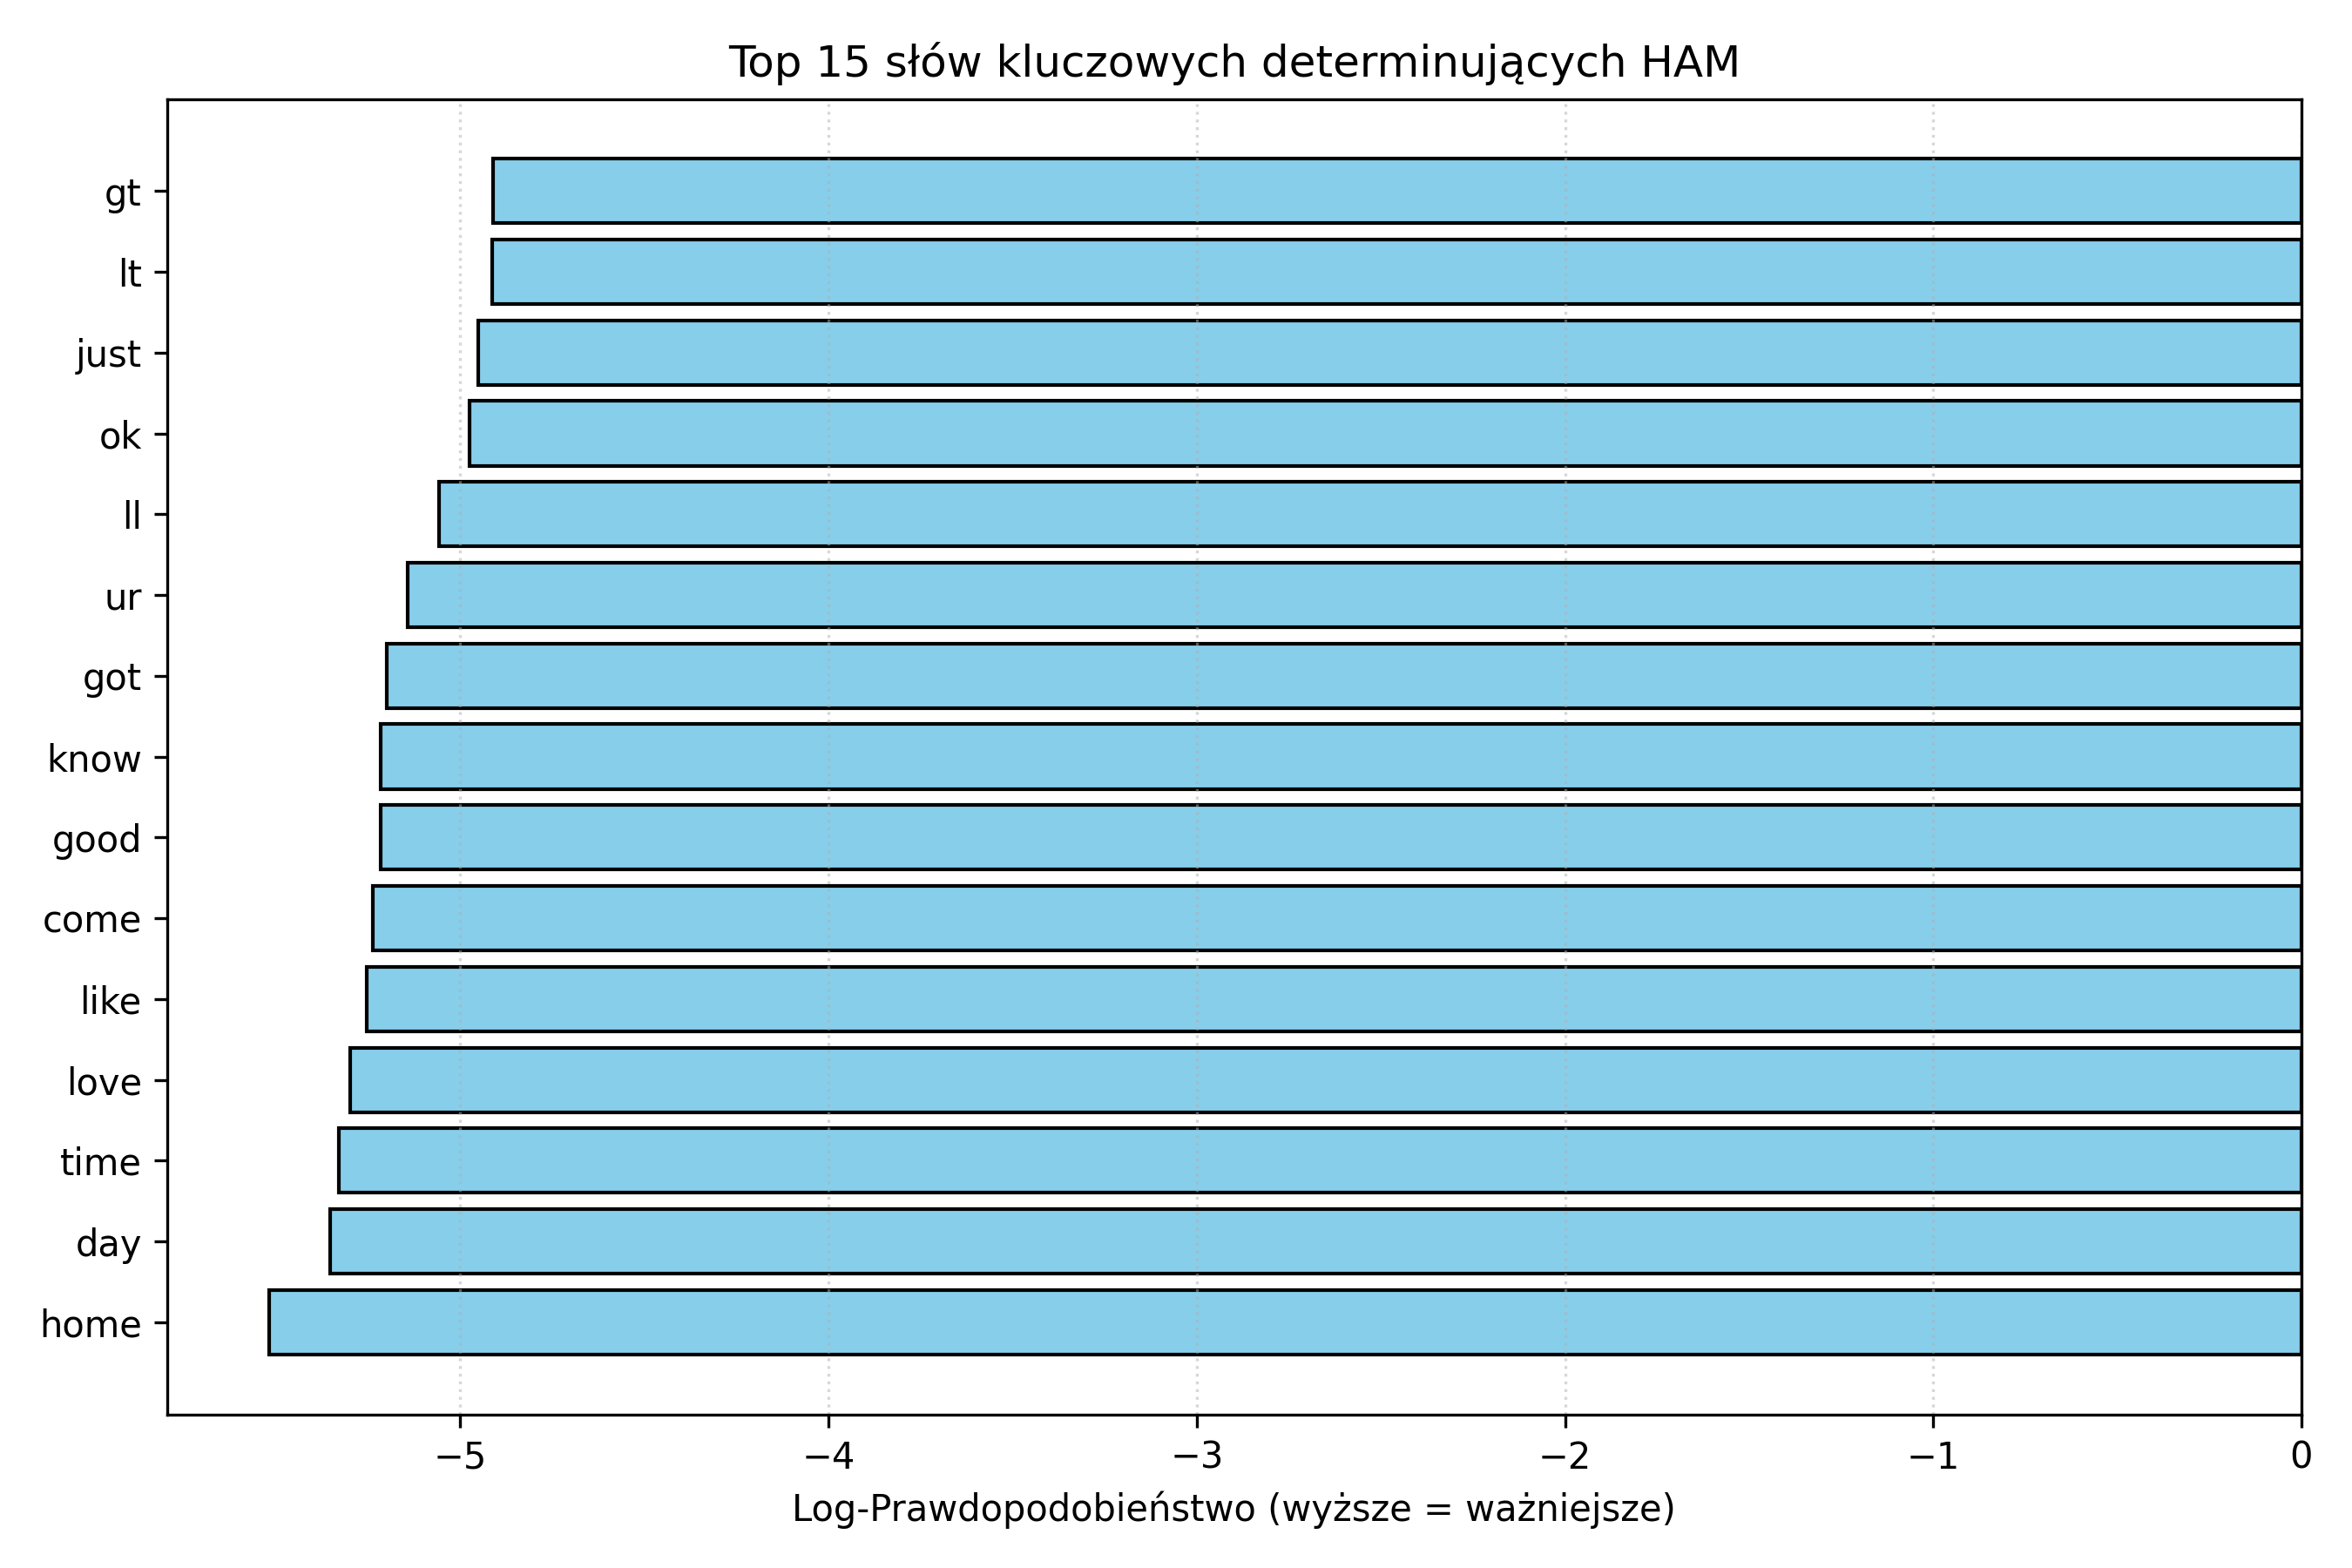
\includegraphics[width=0.6\textwidth]{img/real_ham_features.png}
    \caption{Najważniejsze słowa kluczowe (HAM).}
    \label{fig:ham_feat}
\end{figure}

Klasyfikator osiągnął znakomitą dokładność przekraczającą $98\%$. Wykresy wpływu cech (Rysunek \ref{fig:spam_feat} oraz \ref{fig:ham_feat}) ilustrują wykorzystanie zlogarytmowanego prawdopodobieństwa. Pozwoliło to ominąć błąd niedomiaru arytmetycznego procesora (\textit{arithmetic underflow}) przy analizie długich wiadomości, a jako najsilniejsze indykatory zagrożeń algorytm wyznaczył tokeny marketingowe typu \textit{free, mobile, txt}.

\begin{figure}[H]
    \centering
    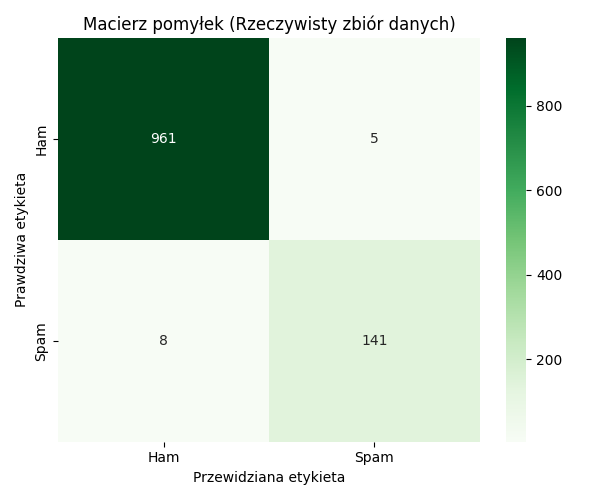
\includegraphics[width=0.65\textwidth]{img/real_bayes_cm.png}
    \caption{Macierz pomyłek dla klasyfikacji SMS.}
    \label{fig:spam_cm}
\end{figure}

\section{Wnioski}
Zrealizowany projekt potwierdza skuteczność wybranych algorytmów analitycznych. Wykazano, że zarówno algorytmy nienadzorowane (klasteryzacja) jak i metody prawdopodobieństwa warunkowego (Naiwny Bayes) dostarczają wysoce precyzyjnych klasyfikacji, pod warunkiem odpowiedniego przygotowania wektorów cech. Z kolei techniki klasy Monte Carlo stanowią potężne i odporne na zakłócenia narzędzie w symulacjach układów o skomplikowanych geometriach.

\newpage
% ==========================================
% BIBLIOGRAFIA
% ==========================================
\begin{thebibliography}{9}

\bibitem{scikit-learn}
Pedregosa, F. et al., \textit{Scikit-learn: Machine Learning in Python}, Journal of Machine Learning Research, vol. 12, pp. 2825-2830, 2011.

\bibitem{uci-wine}
Aeberhard, S., Coomans, D. and De Vel, O., \textit{Comparison of Classifiers in High Dimensional Settings}, Tech. Rep. no. 92-02, Dept. of Computer Science and Dept. of Mathematics and Statistics, James Cook University of North Queensland, 1992. (Dostępne w UCI Machine Learning Repository).

\bibitem{kmedoids}
Kaufman, L., Rousseeuw, P.J., \textit{Partitioning Around Medoids (Program PAM). A Concise Introduction to Classification}, Springer, 1990.

\bibitem{montecarlo}
Metropolis, N., Ulam, S., \textit{The Monte Carlo Method}, Journal of the American Statistical Association, vol. 44, no. 247, pp. 335-341, 1949.

\bibitem{fisher-iris}
Fisher, R. A., \textit{The use of multiple measurements in taxonomic problems}, Annals of Eugenics, vol. 7, pp. 179-188, 1936.

\bibitem{sms-spam}
Almeida, T. A., Gómez Hidalgo, J. M., Yamakami, A., \textit{Contributions to the Study of SMS Spam Filtering: New Collection and Results}, Proceedings of the 2011 ACM Symposium on Document Engineering (DocEng'11), Mountain View, CA, USA, 2011.

\end{thebibliography}

\end{document}